
\subsection{link-analysis}

\textit{Compare different optimization approaches w.r.t. runtime and evaluation metric}

\begin{description}
    \item[grid]
        Does a gridsearch over a subset of $\gamma$ and $\eta$, given a fixed step size. A step size of 1 was used.
    %\item[rand]
        %Randomly samples over a subspace of $\gamma$ and $\eta$, given a fixed number of samples.
    \item[adapt-hill]
        A hill climbing algorithm over both $\gamma$ and $\eta$. It starts with a fixed step size and compares the neighbours. If a local optima is found, the step size is decreased. Continues until a specified function, eta or gamma tolerance has been reached.
    \item[adapt-hill-gamma]
        A hill climbing algorithm over $\gamma$. It starts with a fixed step size and compares the neighbours. If a local optima is found, the step size is decreased. Continues until a specified function or gamma tolerance has been reached. It fixes $\eta = 1$ and after optimizing $\gamma$ checks for $\eta = -1$.
    %\item[sim-ann]
        %Simulated annealing over $\gamma$. Try $\eta = 1$ and $\eta = -1$.
\end{description}


\begin{figure}[h!]
    \centering
    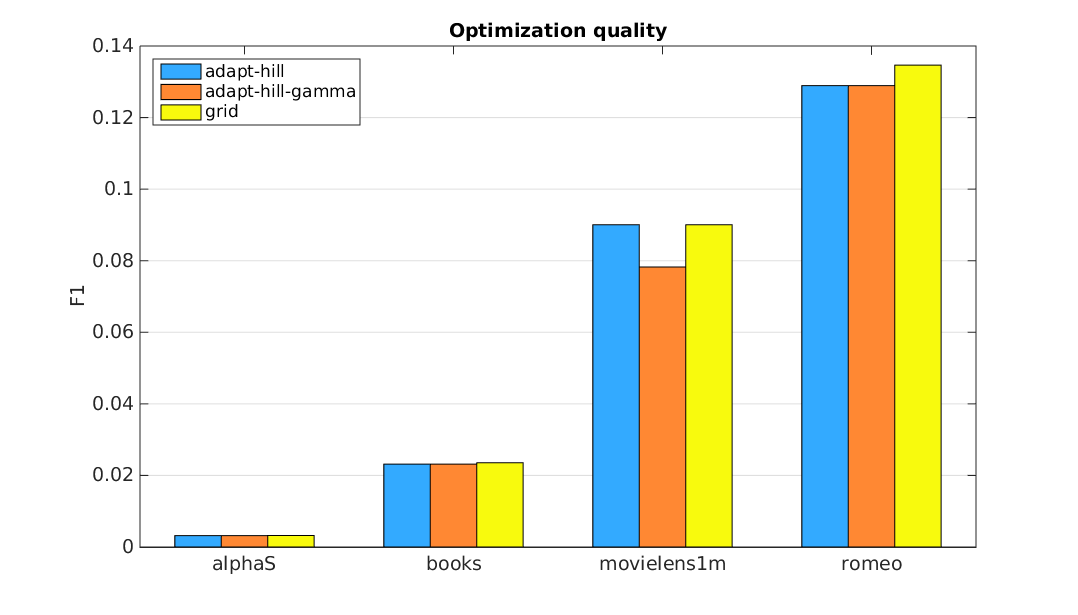
\includegraphics[width=0.9\textwidth]{fig/comp/comp_link_quality.png}
    \caption{Comparison of the recommendation quality given from the parameters found by thedifferent optimization strategies for \textit{link-analysis}.}
\end{figure}

\begin{figure}[h!]
    \centering
    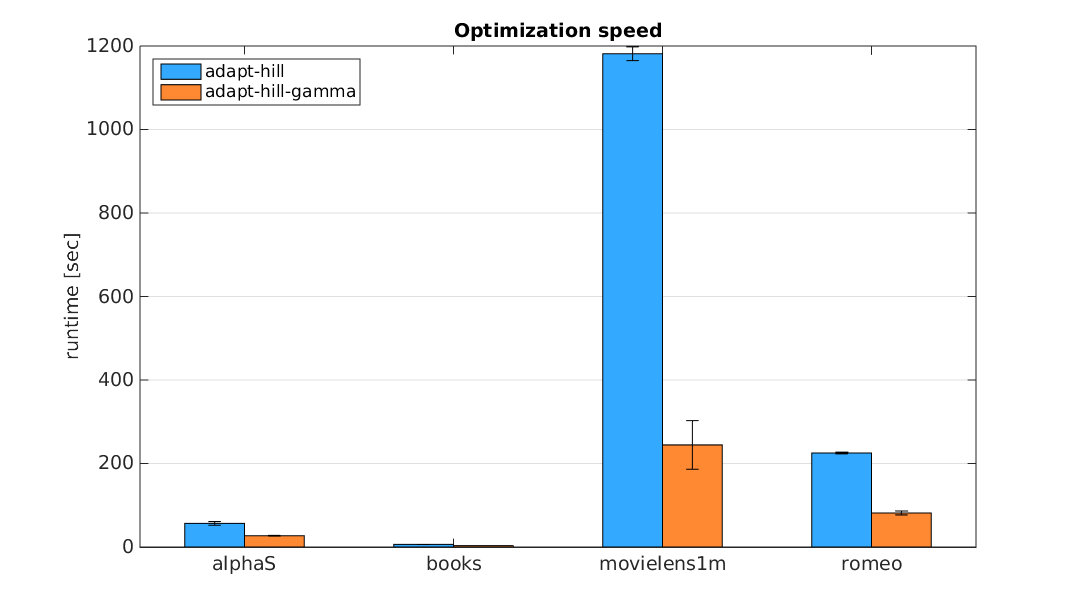
\includegraphics[width=0.9\textwidth]{fig/comp/comp_link_speed.png}
    \caption{Comparison of the runtime of the different optimization strategies for \textit{link-analysis}, given the optimized parameters specified in \appendixref{app:opt_params}.}
\end{figure}

\begin{figure}[h!]
    \centering
    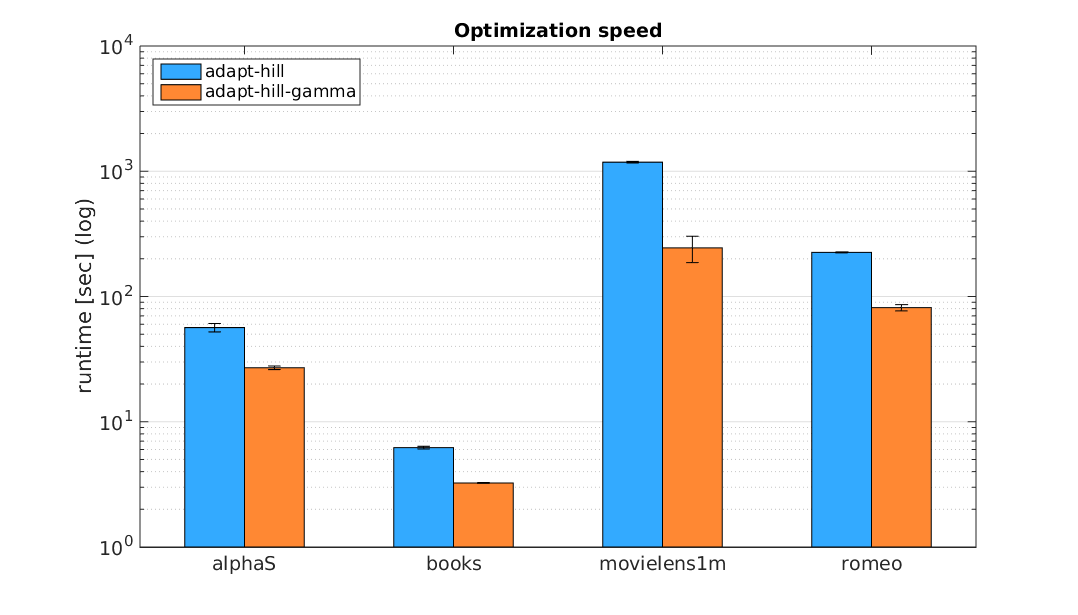
\includegraphics[width=0.9\textwidth]{fig/comp/comp_link_speed_log.png}
    \caption{Comparison of the runtime of the different optimization strategies for \textit{link-analysis}, given the optimized parameters specified in \appendixref{app:opt_params}. In a log scale.}
\end{figure}

\FloatBarrier
